\documentclass[12pt, a4paper]{article}

\usepackage[slovak]{babel}
\usepackage[utf8]{inputenc}
\usepackage[T1]{fontenc}
\usepackage{geometry}
\usepackage{hyperref}
\usepackage{setspace}
\usepackage{subcaption}
\usepackage{afterpage}
\usepackage{graphicx}
\usepackage{csquotes}
\usepackage{longtable}
\usepackage{pdfpages}
\usepackage{expl3}

% Dots in TOC
\usepackage{tocloft}
\renewcommand{\cftsecleader}{\cftdotfill{\cftdotsep}}


\setstretch{1.5}
\widowpenalty10000
\clubpenalty10000
\newsavebox\shield
\usepackage{titlesec}

\usepackage[style=iso-numeric,backend=biber]{biblatex}
\addbibresource{references.bib}
%\AtBeginBibliography{\small}

\geometry{
	a4paper,
	top=2cm,
	left=3cm,
	right=2.5cm,
	bottom=2.5cm
}

\begin{document}
\begin{titlepage}
{\centering
    {\Large Slovenská technická univerzita v Bratislave}\par
    {\Large Fakulta informatiky a informačných technológií}\par
    \vspace{\medskipamount}
    \vfill
    \textbf{\large Bc. Miroslav Hájek}\par
    \vspace{1.5\bigskipamount}
    \Large \textbf{Inteligentné osvetlenie pracovného stola} \\
    \vspace{\bigskipamount}
    {\large Semestrálny projekt}\par
    \vfill
}
\normalsize    
\begin{flushleft}
Máj 2023
\end{flushleft}
\end{titlepage}

\thispagestyle{empty}
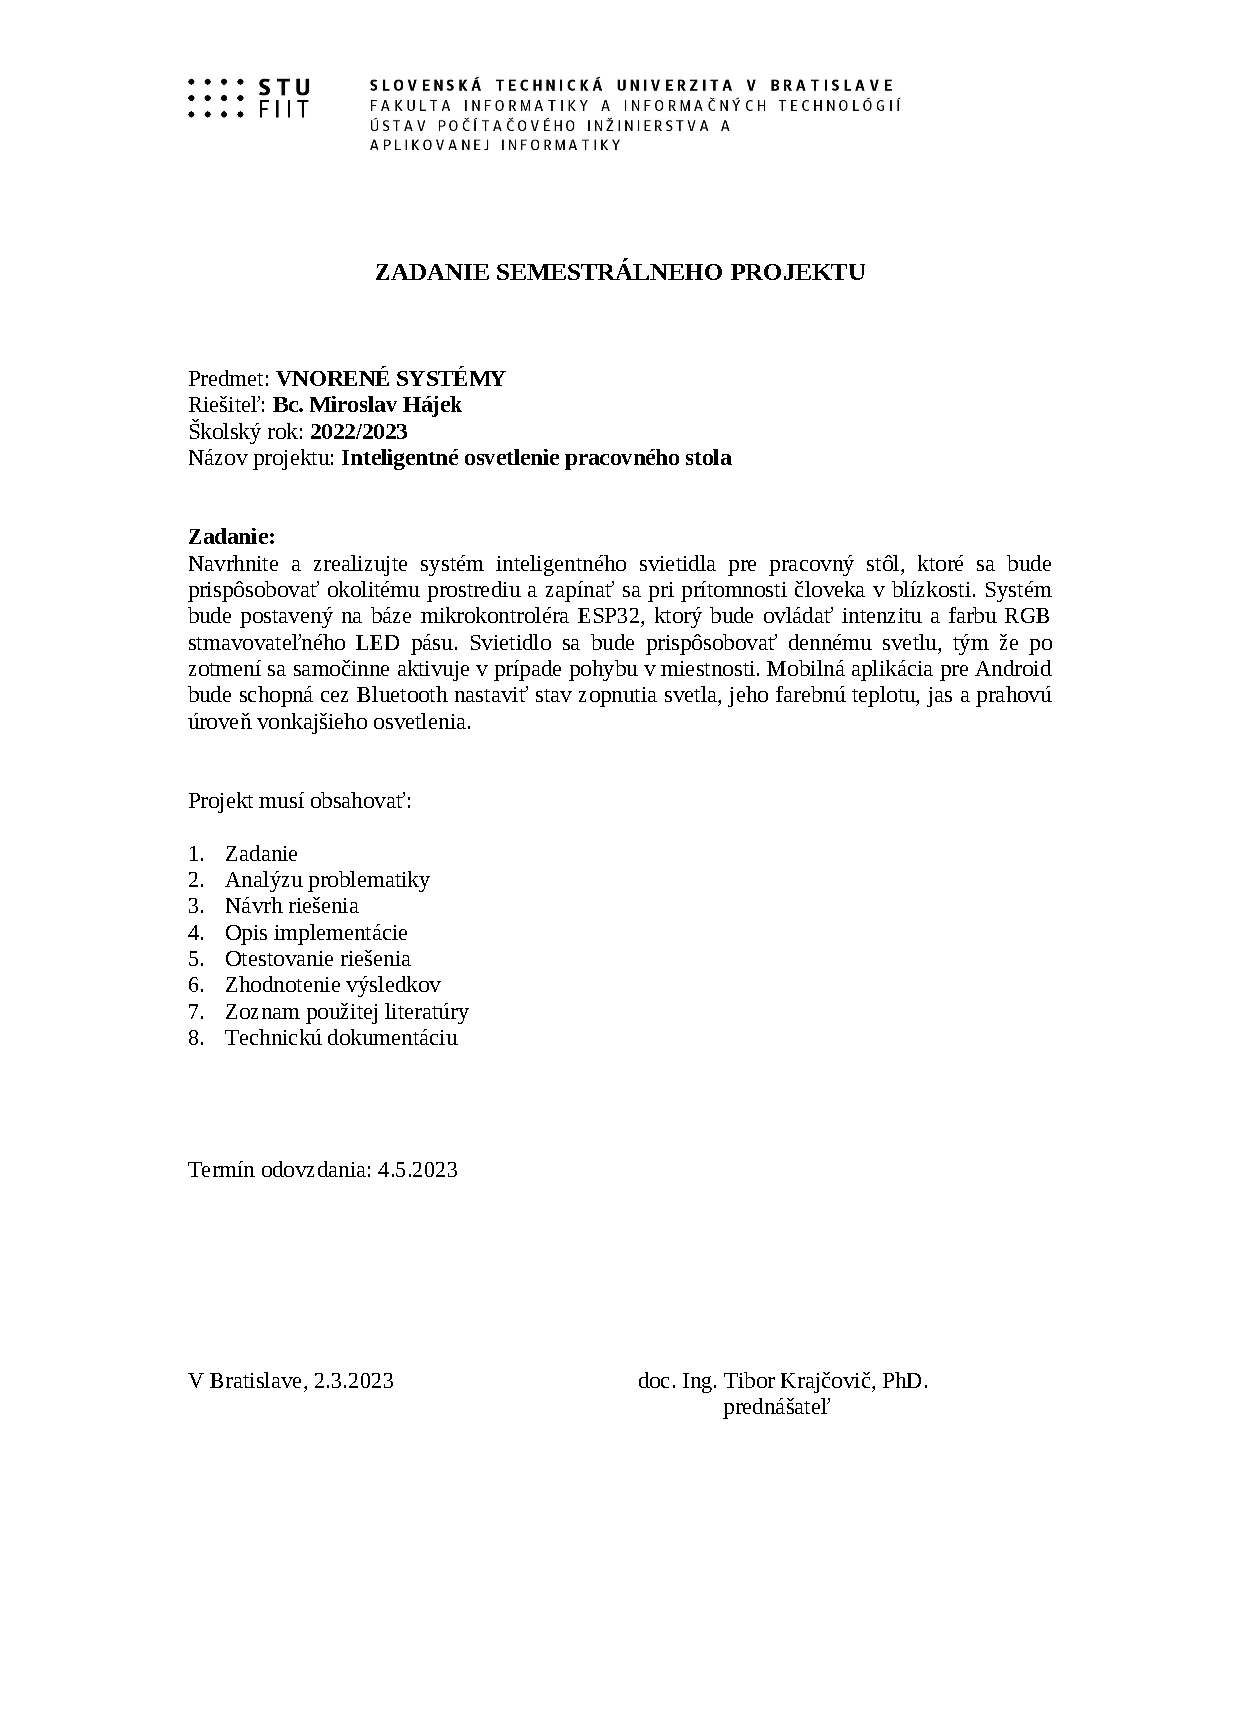
\includepdf[pages=-, scale=1]{zadanie}

\pagenumbering{gobble}
\tableofcontents
\newpage

\pagenumbering{arabic}
\setcounter{page}{1}

\section{Analýza problematiky}
% Moduly a ich cena, driver

\section{Návrh riešenia}
% Schémy
% Wireframe mobilnej aplikácie

\subsection{Opis implementácie}
% ESP-IDF - C kód a drivers
% Android studio

\subsection{Otestovanie riešenia}
% Testovacie scenáre

\section{Zhodnotenie výsledkov}

\printbibliography[title={Literatúra}]
\url{https://tannerhelland.com/2012/09/18/convert-temperature-rgb-algorithm-code.html}
\newpage

\section{Technická dokumentácia}

\end{document}